
%%%%%%%%%%%%%%%%%%%%%%%%%%%%%%%%%%%%%%%%%
% Short Sectioned Assignment LaTeX Template Version 1.0 (5/5/12)
% This template has been downloaded from: http://www.LaTeXTemplates.com
% Original author:  Frits Wenneker (http://www.howtotex.com)
% License: CC BY-NC-SA 3.0 (http://creativecommons.org/licenses/by-nc-sa/3.0/)
%%%%%%%%%%%%%%%%%%%%%%%%%%%%%%%%%%%%%%%%%

%----------------------------------------------------------------------------------------
%	PACKAGES AND OTHER DOCUMENT CONFIGURATIONS
%----------------------------------------------------------------------------------------

\documentclass[paper=a4, fontsize=11pt]{scrartcl} % A4 paper and 11pt font size

% ---- Entrada y salida de texto -----

\usepackage[T1]{fontenc} % Use 8-bit encoding that has 256 glyphs
\usepackage[utf8]{inputenc}
%\usepackage{fourier} % Use the Adobe Utopia font for the document - comment this line to return to the LaTeX default

% ---- Idioma --------

\usepackage[spanish, es-tabla]{babel} % Selecciona el español para palabras introducidas automáticamente, p.ej. "septiembre" en la fecha y especifica que se use la palabra Tabla en vez de Cuadro

% ---- Otros paquetes ----

\usepackage{url} % ,href} %para incluir URLs e hipervínculos dentro del texto (aunque hay que instalar href)
\usepackage{amsmath,amsfonts,amsthm} % Math packages
%\usepackage{graphics,graphicx, floatrow} %para incluir imágenes y notas en las imágenes
\usepackage{graphics,graphicx, float} %para incluir imágenes y colocarlas
\usepackage{movie15}

% Para hacer tablas comlejas
%\usepackage{multirow}
%\usepackage{threeparttable}

%\usepackage{sectsty} % Allows customizing section commands
%\allsectionsfont{\centering \normalfont\scshape} % Make all sections centered, the default font and small caps

\usepackage{fancyhdr} % Custom headers and footers

\pagestyle{fancyplain} % Makes all pages in the document conform to the custom headers and footers
\fancyhead{} % No page header - if you want one, create it in the same way as the footers below
\fancyfoot[L]{} % Empty left footer
\fancyfoot[C]{} % Empty center footer
\fancyfoot[R]{\thepage} % Page numbering for right footer
\renewcommand{\headrulewidth}{0pt} % Remove header underlines
\renewcommand{\footrulewidth}{0pt} % Remove footer underlines
\setlength{\headheight}{13.6pt} % Customize the height of the header

\numberwithin{equation}{section} % Number equations within sections (i.e. 1.1, 1.2, 2.1, 2.2 instead of 1, 2, 3, 4)
\numberwithin{figure}{section} % Number figures within sections (i.e. 1.1, 1.2, 2.1, 2.2 instead of 1, 2, 3, 4)
\numberwithin{table}{section} % Number tables within sections (i.e. 1.1, 1.2, 2.1, 2.2 instead of 1, 2, 3, 4)

\setlength\parindent{0pt} % Removes all indentation from paragraphs - comment this line for an assignment with lots of text

\newcommand{\horrule}[1]{\rule{\linewidth}{#1}} % Create horizontal rule command with 1 argument of height
\usepackage[breaklinks=true]{hyperref}
\usepackage{bookmark}
\usepackage{wasysym}
\usepackage{subcaption}
\usepackage[dvipsnames]{xcolor}
\usepackage{amssymb}
\usepackage{color}
\usepackage{listings}
\usepackage{upgreek} % para poner letras griegas sin cursiva
\usepackage{cancel} % para tachar
\usepackage{mathdots} % para el comando \iddots
\usepackage{mathrsfs} % para formato de letra
\usepackage{stackrel} % para el comando \stackbin
\lstdefinestyle{cmas}
{ %
	language=C++,                % elegir el lenguaje del código
	stringstyle=\color{blue}\ttfamily,,
	basicstyle=\normalsize\ttfamily,       % el tamaño del font a usar para el código
	numbers=left,                   % dónde poner los números de línea 
	numberstyle=\footnotesize,      % tamaño de font usados para los números de línea 
	stepnumber=1,                   % el paso de numeración
	numbersep=8pt,                  % distancia del numero de línea y la línea
	backgroundcolor=\color{white},  % color de fondo, para usarlo hay que agregar  \usepackage{color}
	showspaces=false,               % mostrar espacios en blanco ?
	showstringspaces=false,         % subrayar espacios con cadenas?   
	 showtabs=false,                 % mostrar taba usando cadenas? 
	frame=single,           			% enmarcar el código?  
	tabsize=2,          				% sets default tabsize to 2 spaces?
	keywordstyle=\color{MidnightBlue}\ttfamily\bfseries,
	commentstyle=\color{OliveGreen}\ttfamily,
	morecomment=[l][\color{OliveGreen}]{\#},
	captionpos=b,           % sets the caption-position to bottom?
	breaklines=true,        % sets automatic line breaking?
	breakatwhitespace=false,    % sets if automatic breaks should only happen at whitespace ?
	title=\lstname,
	escapeinside={\%*}{*)}          % if you want to add a comment within your code
}

\lstdefinestyle{payt}
{ %
	language=Python,                % elegir el lenguaje del código
	stringstyle=\color{blue}\ttfamily,,
	basicstyle=\normalsize\ttfamily,       % el tamaño del font a usar para el código
	numbers=left,                   % dónde poner los números de línea 
	numberstyle=\footnotesize,      % tamaño de font usados para los números de línea 
	stepnumber=1,                   % el paso de numeración
	numbersep=8pt,                  % distancia del numero de línea y la línea
	backgroundcolor=\color{white},  % color de fondo, para usarlo hay que agregar  \usepackage{color}
	showspaces=false,               % mostrar espacios en blanco ?
	showstringspaces=false,         % subrayar espacios con cadenas?   
	showtabs=false,                 % mostrar taba usando cadenas? 
	frame=single,           			% enmarcar el código?  
	tabsize=2,          				% sets default tabsize to 2 spaces?
	keywordstyle=\color{MidnightBlue}\ttfamily\bfseries,
	commentstyle=\color{OliveGreen}\ttfamily,
	morecomment=[l][\color{OliveGreen}]{\#},
	captionpos=b,           % sets the caption-position to bottom?
	breaklines=true,        % sets automatic line breaking?
	breakatwhitespace=false,    % sets if automatic breaks should only happen at whitespace ?
	title=\lstname,
	escapeinside={\%*}{*)}          % if you want to add a comment within your code
}

\definecolor{light-gray}{gray}{0.85}

\lstdefinestyle{fich}
{ %
	language=Bash,                % elegir el lenguaje del código
	stringstyle=\color{black}\texttt,
	basicstyle=\normalsize\ttfamily,       % el tamaño del font a usar para el código	
	numbers=left,                   % dónde poner los números de línea 
	numberstyle=\footnotesize,      % tamaño de font usados para los números de línea 
	stepnumber=1,                   % el paso de numeración
	numbersep=8pt,                  % distancia del numero de línea y la línea
	backgroundcolor=\color{light-gray},  % color de fondo, para usarlo hay que agregar  \usepackage{color}
	showspaces=false,               % mostrar espacios en blanco ?
	showstringspaces=false,         % subrayar espacios con cadenas?   
	showtabs=false,                 % mostrar taba usando cadenas? 
%	frame=single,           			% enmarcar el código?  
	tabsize=2,          				% sets default tabsize to 2 spaces?
	captionpos=b,           % sets the caption-position to bottom?
	breaklines=true,        % sets automatic line breaking?
	breakatwhitespace=false,    % sets if automatic breaks should only happen at whitespace ?
	title=\lstname,
	escapeinside={\%*}{*)}          % if you want to add a comment within your code
}

\lstset{literate=
  {á}{{\'a}}1 {é}{{\'e}}1 {í}{{\'i}}1 {ó}{{\'o}}1 {ú}{{\'u}}1
  {Á}{{\'A}}1 {É}{{\'E}}1 {Í}{{\'I}}1 {Ó}{{\'O}}1 {Ú}{{\'U}}1
  {à}{{\`a}}1 {è}{{\`e}}1 {ì}{{\`i}}1 {ò}{{\`o}}1 {ù}{{\`u}}1
  {À}{{\`A}}1 {È}{{\'E}}1 {Ì}{{\`I}}1 {Ò}{{\`O}}1 {Ù}{{\`U}}1
  {ä}{{\"a}}1 {ë}{{\"e}}1 {ï}{{\"i}}1 {ö}{{\"o}}1 {ü}{{\"u}}1
  {Ä}{{\"A}}1 {Ë}{{\"E}}1 {Ï}{{\"I}}1 {Ö}{{\"O}}1 {Ü}{{\"U}}1
  {â}{{\^a}}1 {ê}{{\^e}}1 {î}{{\^i}}1 {ô}{{\^o}}1 {û}{{\^u}}1
  {Â}{{\^A}}1 {Ê}{{\^E}}1 {Î}{{\^I}}1 {Ô}{{\^O}}1 {Û}{{\^U}}1
  {œ}{{\oe}}1 {Œ}{{\OE}}1 {æ}{{\ae}}1 {Æ}{{\AE}}1 {ß}{{\ss}}1
  {ű}{{\H{u}}}1 {Ű}{{\H{U}}}1 {ő}{{\H{o}}}1 {Ő}{{\H{O}}}1
  {ç}{{\c c}}1 {Ç}{{\c C}}1 {ø}{{\o}}1 {å}{{\r a}}1 {Å}{{\r A}}1
  {€}{{\EUR}}1 {£}{{\pounds}}1
  {ñ}{{\~n}}1
}

\hypersetup{
    colorlinks=true,
    linkcolor=black,
    filecolor=magenta,      
    urlcolor=blue,
    pdftitle={ISE: Práctica 3 - Mario Rodríguez Ruiz},
    bookmarks=true,
    citecolor=blue,
}



%----------------------------------------------------------------------------------------
%	TÍTULO Y DATOS DEL ALUMNO
%----------------------------------------------------------------------------------------

\title{	
\normalfont \normalsize 
\textsc{\textbf{Ingeniería de Servidores (2016-2017)} \\ Subgrupo A1 \\ Grado en Ingeniería Informática\\ Universidad de Granada} \\ [25pt] % Your university, school and/or department name(s)
\horrule{0.5pt} \\[0.4cm] % Thin top horizontal rule
\huge Práctica 5: Ajuste del Sistema \\ % The assignment title
\horrule{2pt} \\[0.5cm] % Thick bottom horizontal rule
}

\author{Mario Rodríguez Ruiz} % Nombre y apellidos

\date{\normalsize\today} % Incluye la fecha actual

%----------------------------------------------------------------------------------------
% DOCUMENTO
%----------------------------------------------------------------------------------------

\begin{document}

\maketitle % Muestra el Título

\newpage %inserta un salto de página

\tableofcontents % para generar el índice de contenidos

\listoffigures

\listoftables

\newpage

%----------------------------------------------------------------------------------------
%	Cuestión 1
%----------------------------------------------------------------------------------------

\section{Cuestión 1: SISTEMAS UNIX: SYSCTL Y /PROC}
\subsection{Al modificar los valores del kernel de este modo, no logramos
	que persistan después de reiniciar la máquina. ¿Qué archivo hay que editar
	para que los cambios sean permanentes?}

El archivo que hay que editar para que los cambios sean permanentes es \textbf{/etc/sysctl.conf} \cite{enlace2}, porque en cada inicio del sistema se ejecuta
un script con las configuraciones guardadas en ese archivo\cite{enlace1}. 

Una muestra de lo que puede aparecer en ese fichero es lo que aparece en la Figura \ref{fig:figura1-1}.

\begin{figure}[H] %con el [H] le obligamos a situar aquí la figura
	\centering
	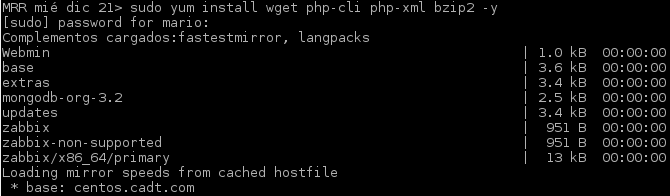
\includegraphics[scale=0.7]{figuras/ejercicio1/figura1-1.png} 
	\caption{Contenido de un fichero \textbf{sysctl.conf} } 
	\label{fig:figura1-1}
\end{figure}

Un ejemplo puede ser el de cambiar el valor del \textbf{swappiness}\cite{enlace3}. Este parámetro controla la tendencia del kernel a insertar los procesos
fuera de la memoria física (swap).
Éste debe tener un valor entre 0 y 100:
\begin{itemize}
	\item \textbf{swappiness = 0} comunica al kernel que evite intercambiar procesos de la memoria física
el mayor tiempo posible.
	\item \textbf{swappiness = 100} le dice al núcleo que cambie de forma brusca los procesos de la memoria física y los mueva a la swap.
\end{itemize}

Por ello, para cambiar este parámetro y hacerlo permanente se insertaría en el fichero
anteriormente mencionado\cite{enlace2} la linea de a continuación\cite{enlace3} y se reflejaría tal y como aparece en la Figura\ref{fig:figura1-2}:
\begin{lstlisting}[style=fich]
vm.swappiness = 20
\end{lstlisting}

\begin{figure}[H] %con el [H] le obligamos a situar aquí la figura
	\centering
	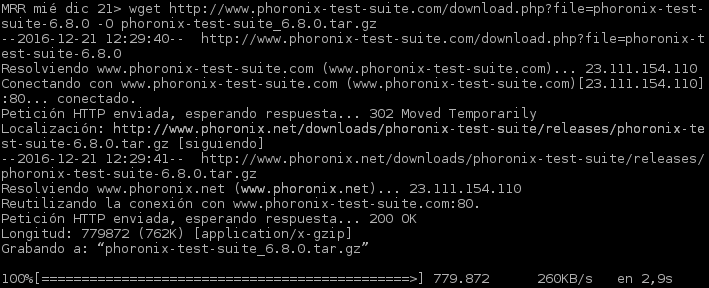
\includegraphics[scale=0.8]{figuras/ejercicio1/figura1-2.png} 
	\caption{Modificación del parámetro swappiness } 
	\label{fig:figura1-2}
\end{figure}

\section{Cuestión 2: SISTEMAS UNIX: SYSCTL Y /PROC}
\subsection{¿Con qué opción se muestran todos los parámetros
	modificables en tiempo de ejecución?}
La opción con la que se muestran todos los parámetros modificables en tiempo de ejecución es la siguiente\cite{enlace1} y puede verse su funcionalidad en la Figura \ref{fig:figura2-1}:
\begin{lstlisting}[style=fich]
$ sysctl -a
\end{lstlisting}
\vspace{-15pt}
O bien, en forma de tabla:
\begin{lstlisting}[style=fich]
$ sysctl -A
\end{lstlisting}
\vspace{-18pt}
\begin{figure}[H] %con el [H] le obligamos a situar aquí la figura
	\centering
	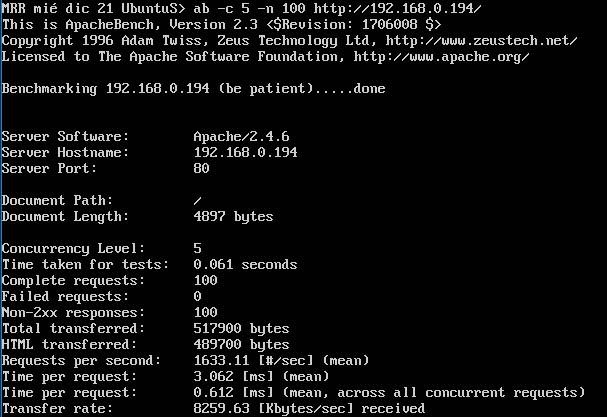
\includegraphics[scale=0.9]{figuras/ejercicio2/figura2-1.png} 
	\caption{Opción para mostrar los parámetros modificables en TE} 
	\label{fig:figura2-1}
\end{figure}
\subsection{Elija dos parámetros y explique, en
	dos líneas, qué función tienen}
Uno de los parámetros que aparecen es \textbf{swappiness}\cite{enlace3} que ya está explicado en la \textbf{Cuestión 1}.

\begin{itemize}
	\item \textbf{kernel.panic}\cite{enlace4}: ante un error del
	núcleo del sistema, se reiniciará pasados tantos segundos como los que tenga asignados. Por defecto está a cero como muestra la figura \ref{fig:figura2-2}.
		\begin{figure}[H] %con el [H] le obligamos a situar aquí la figura
			\centering
			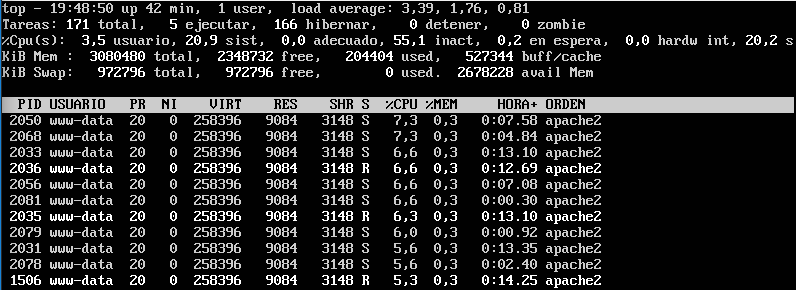
\includegraphics[scale=1]{figuras/ejercicio2/figura2-2.png} 
			\caption{Parámetro \textbf{kernel.panic}} 
			\label{fig:figura2-2}
		\end{figure}
	\item \textbf{kernel.ctrl-alt-del}\cite{enlace5}: este parámetro permite cambiar el funcionamiento de lo que ocurre cuando se pulsa la combinación de teclas \textbf{ctrl-alt-del}. Si valor es cero se llama \textbf{init(1)}, el programa encargado del reinicio
	normal; si el valor es mayor que cero se produce un reinicio inmediato del sistema.
	Por defecto su valor es cero, como muestra la Figura \ref{fig:figura2-3}.
		\begin{figure}[H] %con el [H] le obligamos a situar aquí la figura
			\centering
			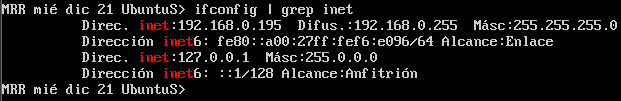
\includegraphics[scale=0.9]{figuras/ejercicio2/figura2-3.png} 
			\caption{Parámetro \textbf{kernel.ctrl-alt-del}} 
			\label{fig:figura2-3}
		\end{figure}
	\item \textbf{vm.stat\_interval}\cite{enlace6}: especifica el intervalo de tiempo en el que se actualizan las estadísticas de memoria virtual
	Por defecto su valor es uno, como muestra la Figura \ref{fig:figura2-4}.
	\begin{figure}[H] %con el [H] le obligamos a situar aquí la figura
		\centering
		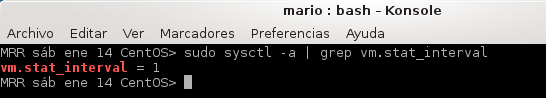
\includegraphics[scale=0.9]{figuras/ejercicio2/figura2-4.png} 
		\caption{Parámetro \textbf{vm.stat\_interval}} 
		\label{fig:figura2-4}
	\end{figure}
\end{itemize}

\section{Cuestión 3: WINDOWS - EDICIÓN DEL REGISTRO}
\subsection{Realice una copia de seguridad del registro y restáurela,
	ilustre el proceso con capturas}

\subsubsection{Copia de seguridad del registro en Windows Server 2012\cite{enlace7}}
	\begin{enumerate}
		\item Pulsando sobre el menú de inicio y escribiendo directamente la palabra \textbf{regedit}, aparecerá un icono como el de la Figura \ref{fig:figura3-1}.
			\begin{figure}[H] %con el [H] le obligamos a situar aquí la figura
				\centering
				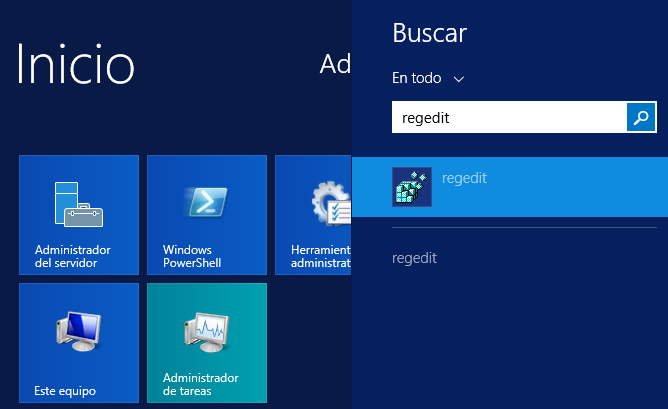
\includegraphics[scale=0.6]{figuras/ejercicio3/figura3-1.png} 
				\caption{Regedit desde el menú de inicio de Windows} 
				\label{fig:figura3-1}
			\end{figure} 
		\item Ahora se muestra una nueva ventana, que será la del Editor del Registro en la que habrá que pulsar sobre \textbf{Archivo} ubicado en la barra de herramientas superior. Su posición se encuentra marcada con una flecha roja en la Figura \ref{fig:figura3-2}.
			\begin{figure}[H] %con el [H] le obligamos a situar aquí la figura
				\centering
				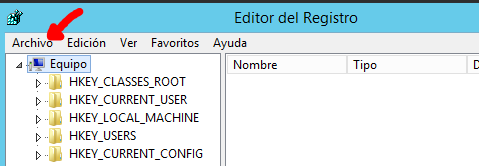
\includegraphics[scale=0.9]{figuras/ejercicio3/figura3-2.png} 
				\caption{Editor del Registro de Windows: Archivo} 
				\label{fig:figura3-2}
			\end{figure}
		\item A continuación se despliega una pestaña con varias opciones entre la que se encuentra \textbf{Exportar}, que es la que hay que elegir, marcada con una flecha roja en la Figura \ref{fig:figura3-3}.
			\begin{figure}[H] %con el [H] le obligamos a situar aquí la figura
				\centering
				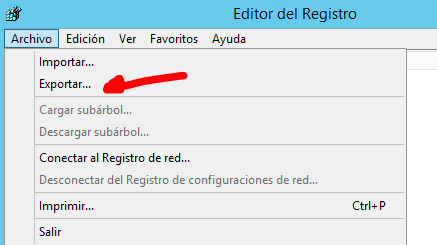
\includegraphics[scale=0.9]{figuras/ejercicio3/figura3-3.png} 
				\caption{Editor del Registro de Windows: Exportar} 
				\label{fig:figura3-3}
			\end{figure}
		\item Por último, aparece una nueva ventana (Figura \ref{fig:figura3-4}) en la que lo único que hay que hacer es elegir un nombre y un destino para el archivo que se creará para la copia de seguridad y pulsar sobre el botón \textbf{Guardar}.
			\begin{figure}[H] %con el [H] le obligamos a situar aquí la figura
				\centering
				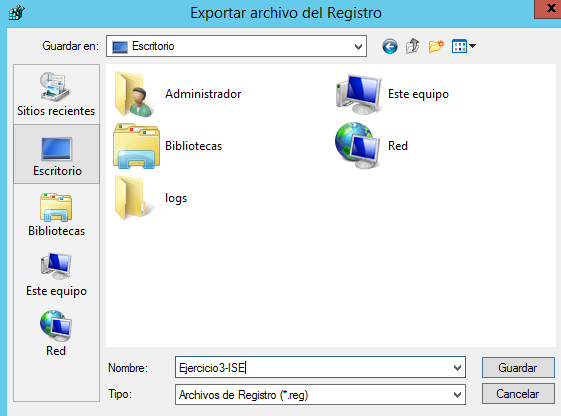
\includegraphics[scale=0.8]{figuras/ejercicio3/figura3-4.png} 
				\caption{Editor del Registro de Windows: Guardar} 
				\label{fig:figura3-4}
			\end{figure}
		\vspace{-15pt}
		\item Llegado a este punto, ya debe de aparecer el archivo de copia en la ubicación que se le haya especificado en el paso anterior. En este caso se ha elegido el \textbf{Escritorio} como destino y \textbf{Ejercicio-ISE} como nombre de fichero, tal y como se muestra en la Figura \ref{fig:figura3-5}.
			\begin{figure}[H] %con el [H] le obligamos a situar aquí la figura
				\centering
				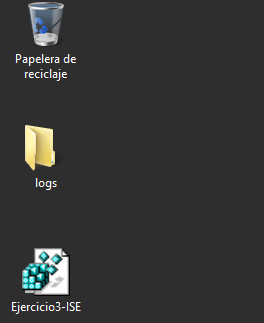
\includegraphics[scale=0.8]{figuras/ejercicio3/figura3-5.png} 
				\caption{Copia realizada con éxito} 
				\label{fig:figura3-5}
			\end{figure}
	\end{enumerate}
\subsubsection{Restauración del registro en Windows Server 2012\cite{enlace7}}
	\begin{enumerate}
		\item Pulsando sobre el menú de inicio y escribiendo directamente la palabra \textbf{regedit}, aparecerá un icono como el de la Figura \ref{fig:figura3-1}.
		
		\item Ahora se muestra una nueva ventana, que será la del Editor del Registro en la que habrá que pulsar sobre \textbf{Archivo} ubicado en la barra de herramientas superior. Su posición se encuentra marcada con una flecha roja en la Figura \ref{fig:figura3-2}.
			\begin{figure}[H] %con el [H] le obligamos a situar aquí la figura
				\centering
				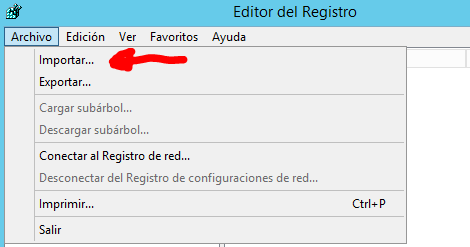
\includegraphics[scale=0.9]{figuras/ejercicio3/figura3-6.png} 
				\caption{Editor del Registro de Windows: Importar} 
				\label{fig:figura3-6}
			\end{figure}
		\item A continuación se despliega una pestaña con varias opciones entre la que se encuentra \textbf{Importar}, que es la que hay que elegir, marcada con una flecha roja en la Figura \ref{fig:figura3-6}.
		
		\item Por último, aparece una nueva ventana (Figura \ref{fig:figura3-7}) en la que lo único que hay que hacer es elegir el archivo donde se encuentre guardada la copia de seguridad y pulsar sobre \textbf{Abrir}. En este caso se ha elegido el fichero creado en el apartado anterior \textbf{Ejercicio3-ISE}.
			\begin{figure}[H] %con el [H] le obligamos a situar aquí la figura
				\centering
				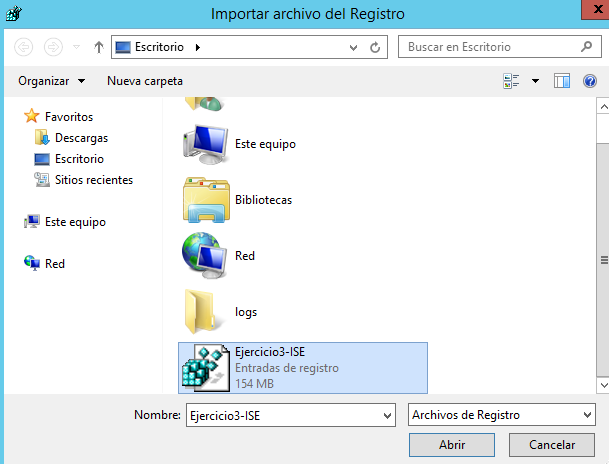
\includegraphics[scale=0.8]{figuras/ejercicio3/figura3-7.png} 
				\caption{Editor del Registro de Windows: Abrir copia} 
				\label{fig:figura3-7}
			\end{figure}		
	\end{enumerate}
	\vspace{-15pt}
	Sin embargo, al terminar todo este proceso se produce un error. Éste se muestra en la Figura \ref{fig:figura3-8} e indica que no es posible realizar la restauración porque hay registros que se encuentran actualmente en uso.
	Se descarta que no se tengan permisos porque también se ha probado a abrir el Editor del Registro en modo administrador (botón derecho sobre regedit y \textbf{ejecutar como administrador}) y se ha obtenido el mismo error.
	
	\begin{figure}[H] %con el [H] le obligamos a situar aquí la figura
		\centering
		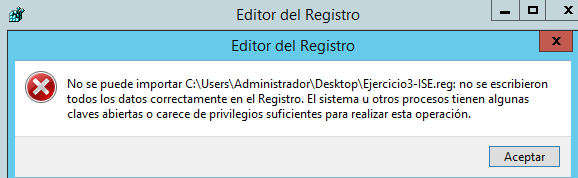
\includegraphics[scale=0.9]{figuras/ejercicio3/figura3-8.png} 
		\caption{Editor del Registro de Windows: Guardar} 
		\label{fig:figura3-8}
	\end{figure}
	Es por ello que para realizar una copia completa se debe de hacer sobre la opción que proporciona Windows en el inicio del sistema: \textbf{Restaurar Sistema} (Al inicio del sistema después de la pantalla de la bios pulsar F8 y a continuación restaurar a un punto anterior).
	
	El problema de esta opción es que la copia de seguridad debe de estar en la carpeta que dispone Windows por defecto para la copia de los registros, como no ocurre en este caso.\\
	
	Para ello existe una herramienta que soluciona este inconveniente: \textbf{SMARegisTry}\cite{enlace8}
		\begin{figure}[H] %con el [H] le obligamos a situar aquí la figura
			\centering
			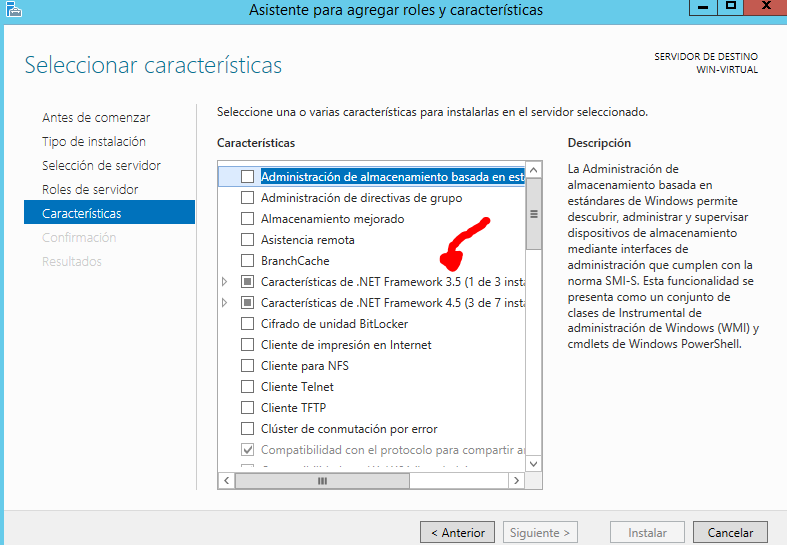
\includegraphics[scale=0.6]{figuras/ejercicio3/figura3-9.png} 
			\caption{Instalación de NET Framework 3.5 en WS 2012} 
			\label{fig:figura3-9}
		\end{figure}
	
	Es necesaria la instalación de NET Framework 3.5 para su ejecución. Éste se consigue mediante la herramienta de Windows Server \textbf{Asistente para agregar roles y características}, como bien se vio en la práctica pasada y que se encuentra en \textbf{Administrador del Servidor $ \rightarrow $ Administrar}. 
	Una vez ahí basta con encontrar la pestaña correspondiente, pulsarla y dar a \textbf{Instalar} como muestra la Figura \ref{fig:figura3-9}.
	\\
	
	Cumplidos ya todos los requisitos para la ejecución de la herramienta, ya es posible su utilización abriéndola a través de su icono correspondiente. La ventana principal es como el contenido de la Figura \ref{fig:figura3-10}.
		\begin{figure}[H] %con el [H] le obligamos a situar aquí la figura
			\centering
			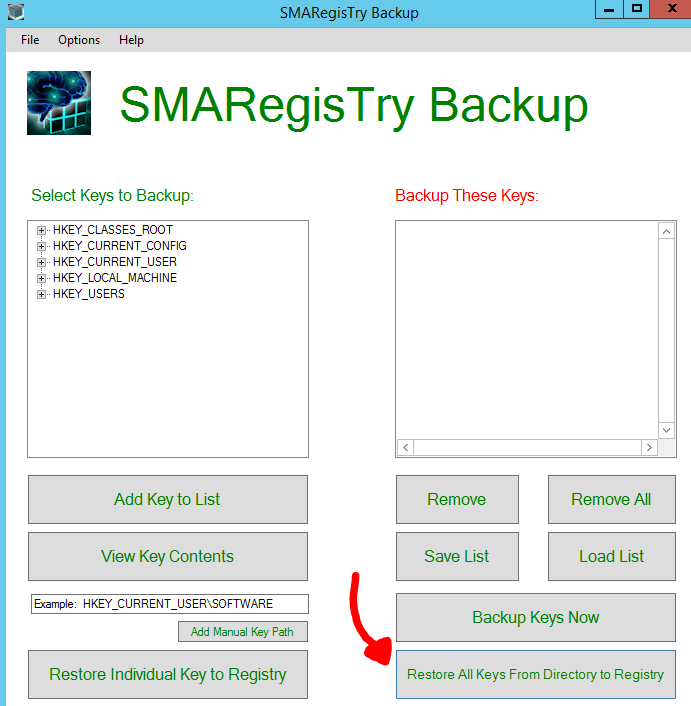
\includegraphics[scale=0.6]{figuras/ejercicio3/figura3-10.png} 
			\caption{SMA Registry} 
			\label{fig:figura3-10}
		\end{figure}
	\vspace{-10pt}
	Para probar su funcionamiento se cambiará el valor de algún registro y posteriormente se importará la copia de seguridad creada con anterioridad a la modificación comprobando que el contenido se ha restaurado correctamente.
	\vspace{5pt}
	
	El registro que se va a cambiar va a ser el de un color de un elemento del escritorio (\textbf{HKEY\_CURRENT\_USER} $ \rightarrow $ \textbf{Control Panel} $ \rightarrow $ \textbf{Desktop} $ \rightarrow $ \textbf{Colors}). El nombre del registro es \textbf{ActiveBorder} y su valor actual es \textbf{212 208 200}.
	\begin{figure}[H] %con el [H] le obligamos a situar aquí la figura
		\centering
		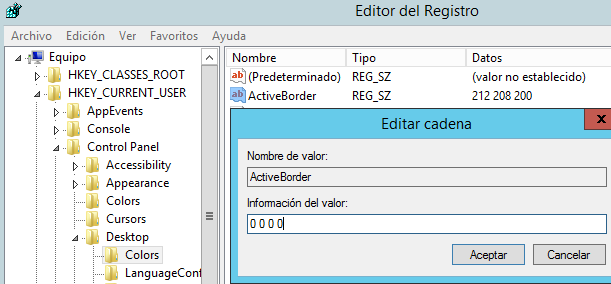
\includegraphics[scale=0.6]{figuras/ejercicio3/figura3-11.png} 
		\caption{Modificación de un registro} 
		\label{fig:figura3-11}
	\end{figure}
	
	Pulsando sobre éste con el botón derecho y a continuación en \textbf{Modificar} puede cambiarse su valor, que en este caso será de \textbf{0 0 0 0} como muestra la Figura \ref{fig:figura3-11}.
	\\
	
	Ahora, para restaurar la copia de seguridad del registro que se creó en el apartado anterior de este mismo ejercicio, se pulsará sobre \textbf{Restore All Keys From Directory to Registry} marcada con una flecha roja en la Figura \ref{fig:figura3-10}.
	
	Por último, aparecerá una ventana para elegir la ubicación de la copia en el sistema y si todo ha salido bien, saldrá un mensaje como el de la Figura \ref{fig:figura3-13}.
		\begin{figure}[H] %con el [H] le obligamos a situar aquí la figura
			\centering
			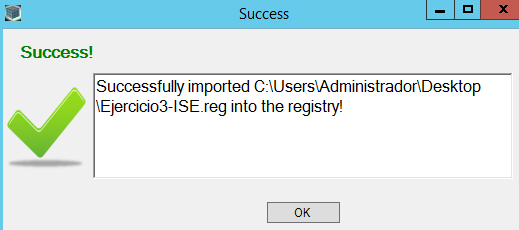
\includegraphics[scale=0.9]{figuras/ejercicio3/figura3-13.png} 
			\caption{Restauración exitosa} 
			\label{fig:figura3-13}
		\end{figure} 
	
	Al volver al Editor del Registro puede verse cómo se ha restaurado el valor del registro que se había modificado, tal y como se ve marcado con una flecha roja en la Figura \ref{fig:figura3-12}.
		\begin{figure}[H] %con el [H] le obligamos a situar aquí la figura
			\centering
			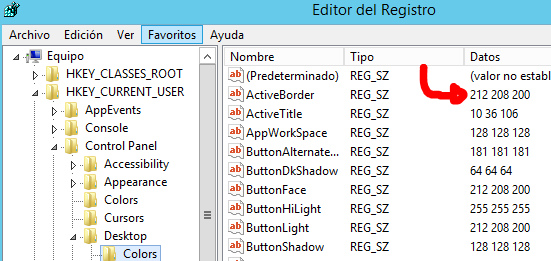
\includegraphics[scale=0.9]{figuras/ejercicio3/figura3-12.png} 
			\caption{Estado del registro tras su restauración} 
			\label{fig:figura3-12}
		\end{figure} 
	\vspace{-5pt}
	La utilización de esta herramienta se debe a que después de buscar el error por diferentes foros de ayuda y faqs de la página de Microsoft no se obtuvo solución alguna y la información que ofrecen sobre el tema es realmente escasa.
\newpage

\subsection{Abra una ventana mostrando el editor del
	registro}
Pulsando sobre el menú de inicio y escribiendo directamente la palabra \textbf{regedit}, aparecerá un icono como el de la Figura \ref{fig:figura3-1}.
\\

La Figura \ref{fig:figura3-14} muestra el Editor del Registro de Windows y, en concreto, el estado del registro \textbf{CursorBlinkRate}.
		\begin{figure}[H] %con el [H] le obligamos a situar aquí la figura
			\centering
			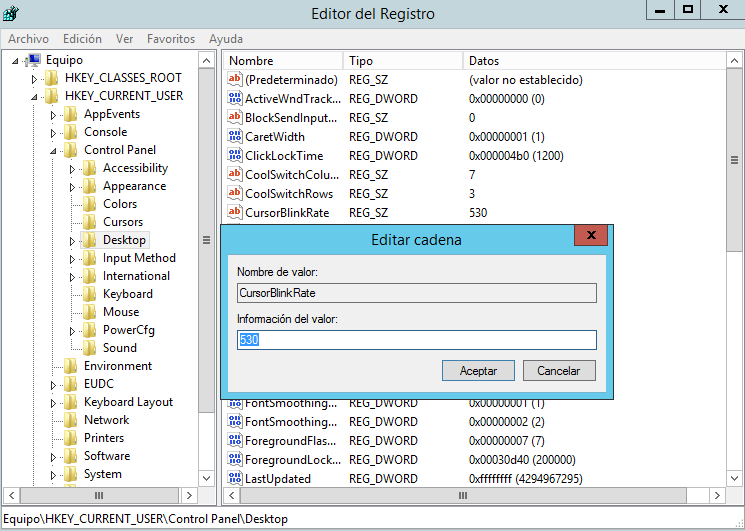
\includegraphics[scale=0.8]{figuras/ejercicio3/figura3-14.png} 
			\caption{Editor del Registro Windows Server 2012} 
			\label{fig:figura3-14}
		\end{figure}

En el apartado anterior de este mismo ejercicio se muestra un ejemplo de modificación de un registro y de su posterior restauración.

\newpage

\section{Cuestión 4: SERVIDOR WEB-APACHE E IIS}

\subsection{Enumere qué elementos se pueden configurar en Apache y en
	IIS para que Moodle funcione mejor}

Una recomendación muy importante antes de optimizar alguna herramienta es la de realizar y ejecutar un benchmark (incluso
varios y hacer una media). Después de hacer las optimizaciones deseadas se volverá a ejecutar el benchmark o benchmarks de igual manera para así comprobar si los resultados son convincentes o si, por el contrario, las prestaciones del servidor han empeorado.

\subsubsection{Mejoras para Apache\cite{enlace9}}
\begin{itemize}
	\item [$ \checkmark $] Ajustar el número máximo de clientes de manera adecuada, atendiendo a la siguiente fórmula:
	
	\textbf{$ MaxClients = MemoriaTotal * 0.8 / UsoMemoriaApache $}
	
	\item [$ \checkmark $] Reducir el número de módulos de Apache al mínimo necesario para así bajar también el uso de 
	memoria.	
	
	\item [$ \checkmark $] Instalar la última versión de Apache. Si se encuentra en Windows Server hacerlo desde \textbf{Apache Lounge} que mejora la estabilidad y el rendimiento.
	
	\item [$ \checkmark $] Reducir la directiva \textbf{MaxRequestsPerChild} del \textbf{httpd.conf} a 20 o 30. Esta directiva
	especifica el número máximo de peticiones que un proceso hijo puede atender.
	
	\item [$ \checkmark $] Para servidores con mucha carga se puede \textbf{desactivar el} \textbf{KeepAlive} (mantiene las conexiones
	TCP abiertas) que reduce latencias pero, por otro lado, consume recursos del servidor.
	Otra opción es la de \textbf{reducir el tiempo del KeepAlive} con la directiva \textbf{KeepAliveTimeout},
	poniéndola en un valor entre 2 y 5 segundos.
	
	\item [$ \checkmark $] Configurar \textbf{DirectoryIndex} para que cargue directamente la página de moodle. De
	esta forma, se evita cualquier tipo de negociación y se reduce la latencia.
	\item [$ \checkmark $] Desactivar \textbf{ExtendedStatus} (si no se están realizando labores de desarrollo o depuración)
	y los modulos \textbf{mod\_info} y \textbf{mod\_status}.
	
	\item [$ \checkmark $] Desactivar el DNS con \textbf{HostnameLookups Off} para evitar latencias.
	
	\item [$ \checkmark $] Reducir la directiva \textbf{TimeOut} a un valor \textbf{entre 30 y 60}. Ésta controla el tiempo
	de espera de Apache para entradas y salidas.
	
	\item [$ \checkmark $] Configurar la directiva \textbf{Options} (Indexes FollowSymLinks) para reducir el uso de disco en lecturas y
	escrituras.	
\end{itemize}

\subsubsection{Mejoras para IIS\cite{enlace9}}
Todas las modificaciones se
realizan bajo la misma ubicación de registro, así que todas las claves que se creen se hará sobre esta ubicación:

\textbf{HKLM\textbackslash SYSTEM\textbackslash
	CurrentControlSet\textbackslash
	 Services\textbackslash
	  Inetinfo\textbackslash
	   Parameters\textbackslash
    }

\begin{itemize}
	\item [$ \checkmark $] Crear una clave \textbf{ListenBackLog} y darle un valor \textbf{entre 2 y 5}. Es el equivalente al
	KeepAliveTimeout de Apache.
	
	\item [$ \checkmark $] Reajustar el tamaño de caché para el fichero de IIS modificando la clave \textbf{MemCacheSize}.
	
	\item [$ \checkmark $] Reajustar el tamaño máximo que un fichero puede tener en caché con \textbf{MaxCachedFileSize}.
	
	\item [$ \checkmark $] Crear una clave llamada \textbf{ObjectCacheTTL} de tipo \textbf{DWORD} que contiene el tiempo en
	mili-segundos que un objeto de caché se mantiene en memoria.
	
\end{itemize}

\section{Cuestión 5: IIS}
\subsection{Ajuste la compresión en el servidor y analice su
	comportamiento usando varios valores para el tamaño de archivo a partir
	del cual comprimir. Para comprobar que está comprimiendo puede usar el
	navegador o comandos como curl (see url) o lynx. Muestre capturas de
	pantalla de todo el proceso}

En primer lugar hay que abrir el administrador de IIS\cite{enlace11}, para ello basta con poner \textbf{inetmgr} en el buscador del menú de inicio, como aparece en la Figura \ref{fig:figura5-4}.
	\begin{figure}[H] %con el [H] le obligamos a situar aquí la figura
		\centering
		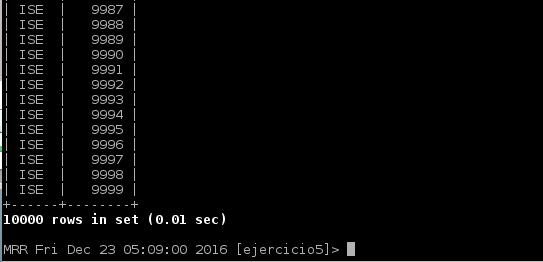
\includegraphics[scale=0.8]{figuras/ejercicio5/figura5-4.png} 
		\caption{Abrir el IIS Manager} 
		\label{fig:figura5-4}
	\end{figure}

Una vez dentro del administrador hay que abrir la herramienta \textbf{Compresión} señalada con una flecha roja en la Figura \ref{fig:figura5-5}.
	\begin{figure}[H] %con el [H] le obligamos a situar aquí la figura
		\centering
		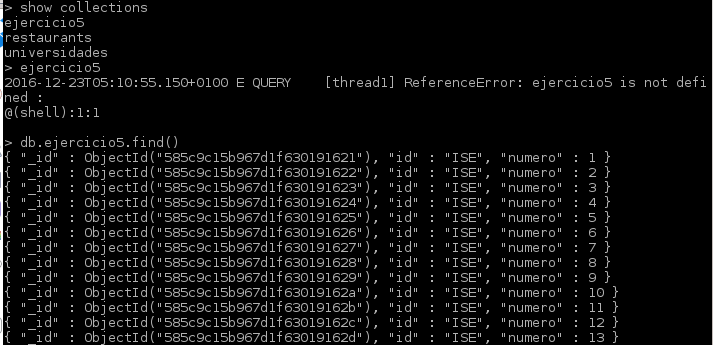
\includegraphics[scale=0.8]{figuras/ejercicio5/figura5-5.png} 
		\caption{Compresión en IIS Manager} 
		\label{fig:figura5-5}
	\end{figure}

A continuación aparecen una serie de opciones que se podrán modificar y que serán válidas después de pulsar el botón \textbf{Aplicar}.
\\

Para comprobar si las respuestas se están comprimiendo, se utilizará la máquina Centos con la herramienta \textbf{Curl}\cite{enlace10}.

La Figura \ref{fig:figura5-2} muestra la dirección IP de Windows Server, que utilizará la máquina Centos para la ejecución de la herramienta antes mencionada.
	\begin{figure}[H] %con el [H] le obligamos a situar aquí la figura
		\centering
		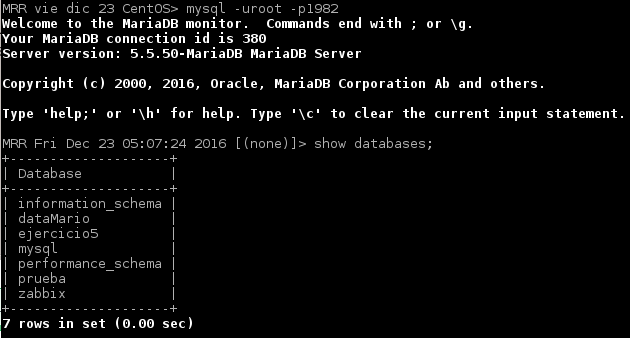
\includegraphics[scale=0.6]{figuras/ejercicio5/figura5-2.png} 
		\caption{Dirección IP de la máquina Windows Server} 
		\label{fig:figura5-2}
	\end{figure}

Como puede verse en la Figura \ref{fig:figura5-3} no se está realizando compresión alguna. Esto se produce porque no se encuentra activa la comprensión de contenido dinámico en el IIS Manager.
	\begin{figure}[H] %con el [H] le obligamos a situar aquí la figura
		\centering
		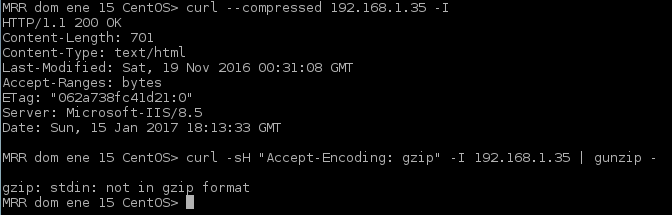
\includegraphics[scale=0.8]{figuras/ejercicio5/figura5-3.png} 
		\caption{Curl desde Centos} 
		\label{fig:figura5-3}
	\end{figure}

Para activar esta característica hay que dirigirse a \textbf{Administrador del servidor} $ \rightarrow $ \textbf{Administrar} $ \rightarrow $ \textbf{Agregar roles y características}.
Una vez dentro de \textbf{Roles de servidor} hay que pulsar sobre \textbf{Compresión de contenido dinámico} señalada con una flecha roja en la Figura \ref{fig:figura5-1}.
	\begin{figure}[H] %con el [H] le obligamos a situar aquí la figura
		\centering
		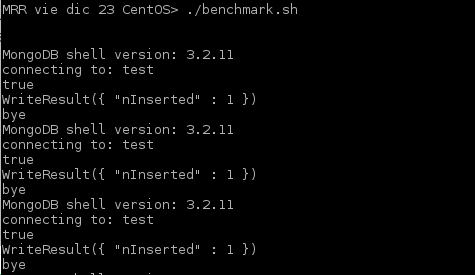
\includegraphics[scale=0.67]{figuras/ejercicio5/figura5-1.png} 
		\caption{Activar compresión de contenido dinámico} 
		\label{fig:figura5-1}
	\end{figure}

Volviendo a IIS Manager y modificando los valores nuevamente bajo esta nueva funcionalidad activa, como muestra la Figura \ref{fig:figura5-6} señaladas en rojo, se aplicarán de nuevo los cambios.
	\begin{figure}[H] %con el [H] le obligamos a situar aquí la figura
		\centering
		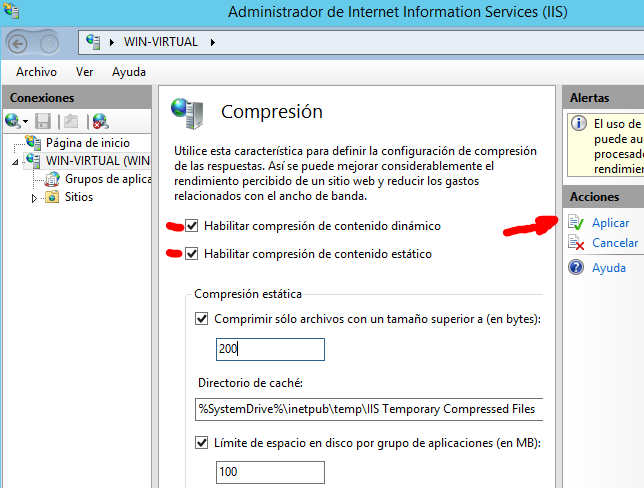
\includegraphics[scale=0.8]{figuras/ejercicio5/figura5-6.png} 
		\caption{Habilitadas las dos comprensiones de contenido} 
		\label{fig:figura5-6}
	\end{figure}
\vspace{-10pt}
De nuevo desde Centos, se ejecuta curl y se obtienen, ahora sí, las respuestas comprimidas como aparece en la Figura \ref{fig:figura5-7}.
	\begin{figure}[H] %con el [H] le obligamos a situar aquí la figura
		\centering
		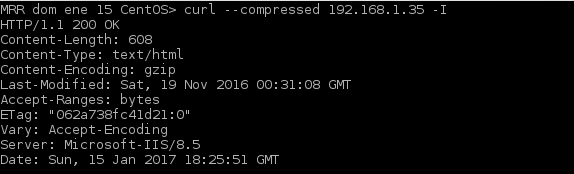
\includegraphics[scale=0.9]{figuras/ejercicio5/figura5-7.png} 
		\caption{Ejecución correcta de curl desde Centos} 
		\label{fig:figura5-7}
	\end{figure}
\vspace{-10pt}
Después de cambiar el valor del tamaño de archivo en varias ocasiones, tanto con valores altos como bajos, no se ha conseguido obtener desde \textbf{curl} resultados distintos del \textbf{Content-Length}.

\section{Cuestión 6: SERVICIOS DE LIBRE ELECCIÓN}

\subsection{Elija un servicio (el que usted quiera) y modifique un parámetro para
	mejorar su comportamiento.}

Se va a proceder a mejorar el comportamiento de \textbf{Apache} en la máquina de \textbf{Ubuntu Server} modificando alguno de los parámetros anteriormente mencionados en la \textbf{Cuestión 4}.

En la Figura \ref{fig:figura6-1} se muestran los módulos que se encuentran actualmente activos para Apache utilizando la orden:
\begin{lstlisting}[style=fich]
> ls /etc/apache2/mods-enabled/
\end{lstlisting}
\vspace{-25pt}
	\begin{figure}[H] %con el [H] le obligamos a situar aquí la figura
		\centering
		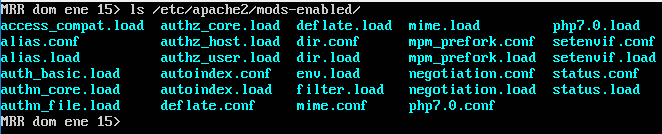
\includegraphics[scale=0.9]{figuras/ejercicio6/figura6-1.png} 
		\caption{Módulos habilitados en Apache en Ubuntu Server} 
		\label{fig:figura6-1}
	\end{figure}
\vspace{-10pt}
En primer lugar, se deshabilitarán los módulos \textbf{setenvif} y \textbf{status} ya que no se están empleando labores de depuración o desarrollo.
\begin{figure}[H] %con el [H] le obligamos a situar aquí la figura
	\centering
	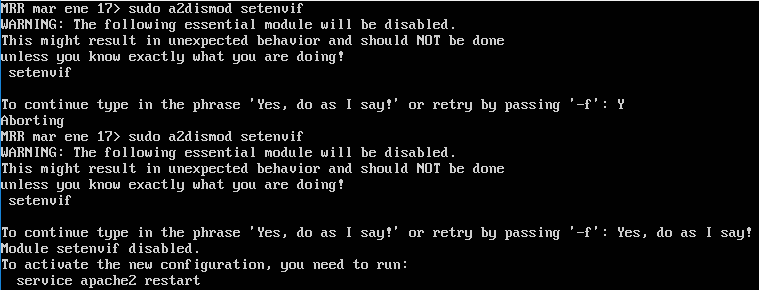
\includegraphics[scale=0.8]{figuras/ejercicio6/figura6-3.png} 
	\caption{Deshabilitación de \textbf{setenvif} Ubuntu Server} 
	\label{fig:figura6-3}
\end{figure}
\vspace{-10pt}
Los comandos para ello son los que aparecen a continuación y su ejecución se muestra en la Figura \ref{fig:figura6-3} y en la Figura \ref{fig:figura6-4}.
\begin{lstlisting}[style=fich]
> sudo a2dismod setenvif
> sudo a2dismod status
\end{lstlisting}
\begin{figure}[H] %con el [H] le obligamos a situar aquí la figura
	\centering
	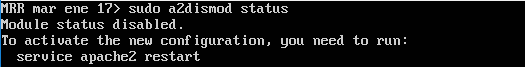
\includegraphics[scale=0.9]{figuras/ejercicio6/figura6-4.png} 
	\caption{Deshabilitación de \textbf{status} Ubuntu Server} 
	\label{fig:figura6-4}
\end{figure}

Además de las modificaciones anteriores, se cambiarán los valores de algunos parámetros del fichero \textbf{/etc/apache2/apache2.conf} para mejorar aún más el rendimiento del servidor.
Estos cambios son los que aparecen a continuación y lo que se muestran señalados con una flecha roja en la Figura \ref{fig:figura6-5}.
\begin{itemize}
	\item [$ \checkmark $] Timeout \textbf{45}
		\item [$ \checkmark $] KeepAlive \textbf{Off}
			\item [$ \checkmark $] KeepAliveTimeout \textbf{2}
\end{itemize}

\begin{figure}[H] %con el [H] le obligamos a situar aquí la figura
	\centering
	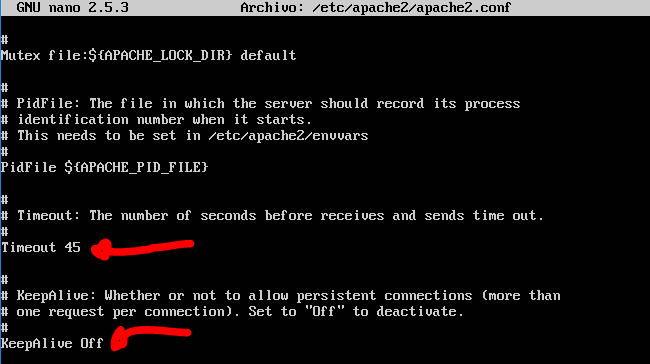
\includegraphics[scale=0.9]{figuras/ejercicio6/figura6-5.png} 
	\caption{Modificación del fichero de Apache2 en Ubuntu Server} 
	\label{fig:figura6-5}
\end{figure}
Los cambios que se han realizado han sido siguiendo el apartado \textbf{Mejoras para Apache} de la \textbf{Cuestión 4} de este mismo archivo. Es por ello por lo que no se ha detallado el por qué de estas modificaciones, evitando así repetir información en un mismo documento.
\subsection{Monitorice el servicio antes y después de
	la modificación del parámetro aplicando cargas al sistema (antes y después)
	mostrando los resultados de la monitorización}

La monitorización del servicio se va a realizar mediante \textbf{Apache Benchmark} (comando \textbf{ab}) desde \textbf{Centos 7} y la orden:
\begin{lstlisting}[style=fich]
$ ab -g datos.csv -c 5 -n 10000 http://direcciónIP/ >> salida.txt
\end{lstlisting}
\vspace{-22pt}
\begin{itemize}
	\item \textbf{-g}: Este parámetro indica que se produzca un volcado de los datos en un fichero especificado para su posterior representación.
	\item \textbf{-n}: Es el número total de peticiones que se van a realizar, que en este caso siempre será \textbf{10000} para que salgan datos útiles con los que poder comparar.
	\item \textbf{-c}: Indica el número de peticiones que se ejecutarán de forma concurrente que en este caso será \textbf{5}.
	\item \textbf{http://direcciónIP/}: Donde \textbf{direccionIP} será la correspondiente a la máquina US, \textbf{192.168.0.196} como muestra la Figura \ref{fig:figura6-2}.
	\item \textbf{$ >> $ salida.txt}: Hace que se guarden todos los resultados finales de la ejecución en un fichero de texto.
\end{itemize}
\vspace{-10pt}	
	\begin{figure}[H] %con el [H] le obligamos a situar aquí la figura
		\centering
		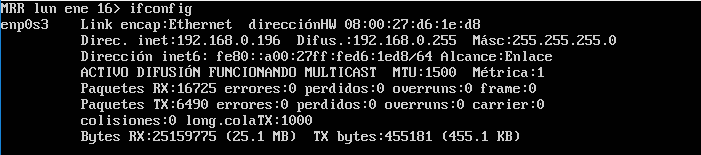
\includegraphics[scale=0.8]{figuras/ejercicio6/figura6-2.png} 
		\caption{Dirección de la máquina Ubuntu Server} 
		\label{fig:figura6-2}
	\end{figure}

La ejecución de dicho comando se realizará tres veces (utilizando el script de a continuación), obteniendo una media al final de éstas con resultados fiables.
\begin{lstlisting}[style=cmas]
#!/bin/bash
max=4
for i in `seq 1 $max`
do
	ab -g datos.csv -c 5 -n 10000 http://192.168.0.196/ >> salida.txt
done
\end{lstlisting}

La Tabla \ref{tab:sinmejora} muestra los resultados de las tres ejecuciones, así como los promedios de éstas obtenidas con \textbf{ab} sobre Apache antes de modificar los parámetros para su optimización.
\\

En este caso, lo que se valora para su posterior comparación son los resultados del tiempo total (\textbf{17,822 s}), de las solicitudes por segundo (\textbf{561,623}), del tiempo por solicitud (\textbf{1,782 ms}) y el ratio de transferencia (\textbf{6355,98 KBytes/sec}).

% Table generated by Excel2LaTeX from sheet 'Hoja1'
\begin{table}[H]
	\centering
	\begin{tabular}{lrrrr}
		\textbf{Ubuntu Server} & \multicolumn{1}{l}{\textbf{Ejecución 1}} & \multicolumn{1}{l}{\textbf{Ejecución 2}} & \multicolumn{1}{l}{\textbf{Ejecución 3}} & \multicolumn{1}{l}{\textbf{Media}} \\
		\midrule
		\textbf{Server Software} & Apache/2.4.18 & Apache/2.4.18 & Apache/2.4.18 &  \\
		\textbf{Server Hostname} & 192.168.0.196 & 192.168.0.196 & 192.168.0.196 &  \\
		\textbf{Server Port} & 80    & 80    & 80    &  \\
		\textbf{Document Path} & /     & /     & /     &  \\
		\textbf{Document Length (bytes)} & 11321 & 11321 & 11321 &  \\
		\textbf{Concurrency Level} & 5       & 5       & 5       &  \\
		\textbf{Time taken for tests (seconds)} & 17,963 & 17,331 & 18,173 & \textbf{17,822} \\
		\textbf{Complete requests} & 10000 & 10000 & 10000 &  \\
		\textbf{Failed requests} & 0     & 0     & 0     &  \\
		\textbf{Write errors} & 0     & 0     & 0     &  \\
		\textbf{Total transferred [bytes]} & 115950000 & 115950000 & 115950000 &  \\
		\textbf{HTML transferred [bytes]} & 113210000 & 113210000 & 113210000 &  \\
		\textbf{Requests per second [\#/sec]} & 556,690 & 577,010 & 550,270 & \textbf{561,323} \\
		\textbf{Time per request (ms)} & 1,796 & 1,733 & 1,817 & \textbf{1,782} \\
		\textbf{Transfer rate [Kbytes/sec]} & 6303,49 & 6533,61 & 6230,84 & \textbf{6355,98} \\
	\end{tabular}%
	\caption{Resultados de \textbf{ab} para Apache sin mejoras}
	\label{tab:sinmejora}%
\end{table}%		

La Tabla \ref{tab:porcentajeSin} ofrece el porcentaje de solicitudes atendidas dentro de un tiempo determinado de las tres ejecuciones, así como el promedio de éstas, obtenidas con \textbf{ab} sobre Apache antes de modificar los parámetros para su optimización.

% Table generated by Excel2LaTeX from sheet 'Hoja1'
\begin{table}[H]
	\centering
	\begin{tabular}{rrrrr}
		\multicolumn{1}{l}{\textbf{Ubuntu Server}} & \multicolumn{1}{l}{\textbf{Ejecución 1}} & \multicolumn{1}{l}{\textbf{Ejecución 2}} & \multicolumn{1}{l}{\textbf{Ejecución 3}} & \multicolumn{1}{l}{\textbf{Media}} \\
		\midrule
		\textbf{50\%} & 1     & 1     & 2     & \textbf{1,33} \\
		\textbf{66\%} & 2     & 2     & 2     & \textbf{2,00} \\
		\textbf{75\%} & 2     & 2     & 2     & \textbf{2,00} \\
		\textbf{80\%} & 2     & 2     & 2     & \textbf{2,00} \\
		\textbf{90\%} & 3     & 3     & 3     & \textbf{3,00} \\
		\textbf{95\%} & 3     & 3     & 3     & \textbf{3,00} \\
		\textbf{98\%} & 3     & 3     & 3     & \textbf{3,00} \\
		\textbf{99\%} & 3     & 3     & 4     & \textbf{3,33} \\
		\textbf{100\%} & 37    & 70    & 57    & \textbf{54,67} \\
	\end{tabular}%	
	\caption{Porcentaje de las respuestas sin mejora}
	\label{tab:porcentajeSin}%
\end{table}%

La Tabla \ref{tab:mejora} muestra los resultados de las tres ejecuciones, así como los promedios de éstas obtenidas con \textbf{ab} sobre Apache después de modificar los parámetros para su optimización.
\\

En este caso, lo que se valora para su posterior comparación con los resultados anteriores es: el tiempo total (\textbf{6,651 s}), de las solicitudes por segundo (\textbf{1432,063}), del tiempo por solicitud (\textbf{0,699 ms}) y el ratio de transferencia (\textbf{16215,61 KBytes/sec}).

% Table generated by Excel2LaTeX from sheet 'Hoja1'
\begin{table}[H]
	\centering
	\begin{tabular}{lrrrr}
		\textbf{Ubuntu Server} & \multicolumn{1}{l}{\textbf{Ejecución 1}} & \multicolumn{1}{l}{\textbf{Ejecución 2}} & \multicolumn{1}{l}{\textbf{Ejecución 3}} & \multicolumn{1}{l}{\textbf{Media}} \\
		\midrule
		\textbf{Server Software} & Apache/2.4.18 & Apache/2.4.18 & Apache/2.4.18 &  \\
		\textbf{Server Hostname} & 192.168.0.196 & 192.168.0.196 & 192.168.0.196 &  \\
		\textbf{Server Port} & 80    & 80    & 80    &  \\
		\textbf{Document Path} & /     & /     & /     &  \\
		\textbf{Document Length (bytes)} & 11321 & 11321 & 11321 &  \\
		\textbf{Concurrency Level} & 5     & 5     & 5     &  \\
		\textbf{Time taken for tests (seconds)} & 5,855 & 7,027 & 7,070 & \textbf{6,651} \\
		\textbf{Complete requests} & 10000 & 10000 & 10000 &  \\
		\textbf{Failed requests} & 0     & 0     & 0     &  \\
		\textbf{Write errors} & 0     & 0     & 0     &  \\
		\textbf{Total transferred [bytes]} & 115950000 & 115950000 & 115950000 &  \\
		\textbf{HTML transferred [bytes]} & 113210000 & 113210000 & 113210000 &  \\
		\textbf{Requests per second [\#/sec]} & 1458,750 & 1423,080 & 1414,360 & \textbf{1432,063} \\
		\textbf{Time per request (ms)} & 0,686 & 0,703 & 0,707 & \textbf{0,699} \\
		\textbf{Transfer rate [Kbytes/sec]} & 16517,80 & 16113,89 & 16015,14 & \textbf{16215,61} \\
	\end{tabular}%	
	\caption{Resultados de \textbf{ab} para Apache con mejoras}
	\label{tab:mejora}%
\end{table}%

La Tabla \ref{tab:mejora2} ofrece el porcentaje de solicitudes atendidas dentro de un tiempo determinado de las tres ejecuciones, así como el promedio de éstas, obtenidas con \textbf{ab} sobre Apache después de modificar los parámetros para su optimización.

% Table generated by Excel2LaTeX from sheet 'Hoja1'
\begin{table}[H]
	\centering
	\begin{tabular}{rrrrr}
		\multicolumn{1}{l}{\textbf{Ubuntu Server}} & \multicolumn{1}{l}{\textbf{Ejecución 1}} & \multicolumn{1}{l}{\textbf{Ejecución 2}} & \multicolumn{1}{l}{\textbf{Ejecución 3}} & \multicolumn{1}{l}{\textbf{Media}} \\
		\midrule
		\textbf{50\%} & 3     & 3     & 3     & \textbf{3,00} \\
		\textbf{66\%} & 3     & 4     & 4     & \textbf{3,67} \\
		\textbf{75\%} & 4     & 4     & 4     & \textbf{4,00} \\
		\textbf{80\%} & 4     & 4     & 4     & \textbf{4,00} \\
		\textbf{90\%} & 4     & 5     & 5     & \textbf{4,67} \\
		\textbf{95\%} & 5     & 5     & 5     & \textbf{5,00} \\
		\textbf{98\%} & 7     & 6     & 7     & \textbf{6,67} \\
		\textbf{99\%} & 8     & 8     & 8     & \textbf{8,00} \\
		\textbf{100\%} & 66    & 20    & 59    & \textbf{48,33} \\
	\end{tabular}%
	\caption{Porcentaje de las respuestas con mejora}
	\label{tab:mejora2}%
\end{table}%

La Tabla \ref{tab:comparativa} muestra un resumen que contiene una comparativa de los resultados obtenidos con los dos tipos distintos de ejecuciones (Ejecución con y sin mejoras).

% Table generated by Excel2LaTeX from sheet 'Hoja1'
\begin{table}[H]
	\centering
	\begin{tabular}{lrrr}
		\textbf{Ubuntu Server} & \multicolumn{1}{l}{\textbf{Sin mejoras}} & \multicolumn{1}{l}{\textbf{Con mejoras}} & \multicolumn{1}{l}{\textbf{Diferencia}} \\
		\midrule
		\textbf{Time taken for tests (seconds)} & 17,822 & 6,651 & 2,6797815 \\
		\textbf{Requests per second [\#/sec]} & 561,323 & 1432,063 & 2,5512272 \\
		\textbf{Time per request (ms)} & 1,782 & 0,699 & 2,5505725 \\
		\textbf{Transfer rate [Kbytes/sec]} & 6355,98 & 16215,61 & 2,5512272 \\
	\end{tabular}%
	\caption{Tabla comparativa de los resultados}	
	\label{tab:comparativa}%
\end{table}%

En ésta, puede observarse cómo los resultados que tienen que ver con tiempo son casi tres veces menores en el Apache que se ha optimizado. 
\\

Por otro lado, los resultados obtenidos en relación con las transferencias son casi tres veces más altos. Lo que quiere decir que se hacen tres veces más de solicitudes por segundo y existe un ratio de transferencia casi tres veces más elevado.
\\

Para concluir, hay que decir que es conveniente \textbf{realizar una personalización} de las características de configuración del servidor. Porque como puede verse en los resultados obtenidos, no siempre los valores \textbf{por defecto} son los más adecuados, ya que \textbf{utilizan más recursos} de los que de verdad son necesarios.

\newpage

%----------------------------------------------------------------------------------------
%	Referencias
%----------------------------------------------------------------------------------------
%------------------------------------------------

\bibliography{citas} %archivo citas.bib que contiene las entradas 
\bibliographystyle{plain} % hay varias formas de citar

\end{document}
